\section{Velvet Interlinks}\label{sec:velvet}
More recently, velvet forks have been introduced~\cite{velvet}. In a
velvet fork, blocks created by upgraded miners (called \emph{velvet blocks}) are
accepted by unupgraded miners as in a soft fork. Additionally, blocks created by
unupgraded miners are also accepted by upgraded miners. This allows the protocol
to upgrade even if only a minority of miners chooses to upgrade. To maintain
backwards compatibility and to avoid causing forks, the additional data included
in a block is \emph{advisory} and must be accepted whether it exists or not.
Even if the additional data is invalid or malicious, upgraded nodes (in this
context also called \emph{velvet nodes}) are forced to accept the blocks. The
simplest approach to velvet fork the chain for interlinking purposes is to have
upgraded miners include the interlink pointer in the blocks they produce, but
accept blocks with missing or incorrect interlinks. As we show in the next
section, this approach is flawed and susceptible to unexpected attacks. A
surgical change in the way velvet blocks are produced is necessary to achieve
proper security.

In a velvet fork, only a minority of honest parties needs to support the protocol
changes. We refer to this percentage as the ``velvet parameter''.

\begin{definition}[Velvet Parameter]
	The \emph{velvet parameter} $g$ is defined as the percentage of honest parties
	that have upgraded to the new protocol. The absolute number of honest upgraded
	parties is denoted $n_h$ and it holds that
	$n_h = g (n - t)$.
	\label{defn:velvet_honest_majority}
\end{definition}

Velvet forks maintain backwards and forwards compatibility. This requires any
block produced by upgraded miners to be accepted by unupgraded nodes (as in a
soft fork), but also blocks produced by unupgraded miners to be accepted by
upgraded nodes. For the particular case of superblock NIPoPoWs under velvet
forks, upgraded miners must include the interlink data structure within their
blocks, but must also accept blocks missing the interlink structure or
containing an invalid interlink. Unupgraded honest nodes will produce blocks
that contain no interlink, while upgraded honest nodes will produce blocks that
contain truthful interlinks. Therefore, any block with invalid interlinks will
be adversarially generated. However, such blocks cannot be rejected by the
upgraded nodes, as that would give the adversary an opportunity to cause a hard
fork.

A block generated by the adversary can thus contain arbitrary data in the
interlink and yet be adopted by an honest party. Because the honest prover is an
upgraded full node, it can determine what the correct interlink pointers are by
examining the whole previous chain, and can thus deduce whether a block contains
invalid interlink data. In that case, the prover can simply treat such blocks as
unupgraded. In the context of the attack that will be presented in the following
section, we examine the case where the adversary includes false interlink
pointers.

In any velvet protocol, a specific portion within a block, which is treated as
a comment by unupgraded nodes, is reused to contain auxiliary data by upgraded
miners. Because these auxiliary data can be deterministically calculated,
upgraded full nodes can verify the authenticity of the data in a new block they
receive. We distinguish blocks based on whether they follow the velvet protocol
rules or they deviate from them.

\begin{definition}[Smooth and Thorny blocks]
A block in a velvet protocol upgrade is called \emph{smooth} if it contains
auxiliary data and the data corresponds to the honest upgraded protocol. A block
is called \emph{thorny} if it contains auxiliary data, but the data differs from
the honest upgraded protocol. A block can be neither smooth nor thorny if it
does not contain auxiliary data.
\end{definition}

In the case of velvet forks for interlink purposes, the auxiliary data consists
of the Merkle Tree containing the interlink pointers to the most recent
superblock ancestor at every level $\mu$.

\noindent
\textbf{A na\"ive velvet scheme.}
In previous work~\cite{nipopows}, it was conjectured that superblock NIPoPoWs
remain secure under a velvet fork. We call this scheme the \emph{Na\"ive Velvet
NIPoPoW} protocol, because it is not dissimilar from the NIPoPoW protocol in the
soft fork case. In particular, the na\"ive velvet NIPoPoW protocol that was put
forth works as follows. Each upgraded honest miner attempts to mine a block $b$
that includes interlink pointers in the form of a Merkle Tree included in its
coinbase transaction. For each level $\mu$, the interlink contains a pointer to
the most recent among all the anecestors of $b$ that have achieved at least
level $\mu$, regardless of whether the referenced block is upgraded or not and
regardless of whether its interlinks are valid. Unupgraded honest nodes will
keep mining blocks on the chain as usual; because the status of a block as
superblock does not require it to be mined by an upgraded miner, the unupgraded
miners contribute mining power to the creation of superblocks as desired.

The prover in the na\"ive velvet NIPoPoWs then worked as follows. The honest
prover constructed the NIPoPoW proof $\pi \chi$ as usual by selecting certain
superblocks from his chain $\chain$ as representatives in $\pi$ and by setting
$\chi = \chain[-k{:}]$. The outstanding issue in this case, however, is that
these blocks in $\pi$ do not form a chain because, while superblocks, some of
them may not be upgraded and they may not contain any pointers (or they may
contain invalid pointers). The honest prover needs to provide a connection
between two consecutive blocks $\pi[i + 1]$ and $\pi[i]$ in the superchain, and
suppose $\pi[i]$ is the most recent $\mu$-superblock preceding $\pi[i + 1]$. The
block $\pi[i + 1]$ is a superblock and exists at some position $j$ in the
underlying chain $\chain$ of the prover, i.e., at $\pi[i + 1] = \chain[j]$. If
$\chain[j]$ is a smooth block, then the interlink pointer at level $\mu$ within
it can be used directly. Otherwise, the prover used the \emph{previd} pointer of
$\pi[i + 1] = \chain[j]$ to repeatedly reach the parents of $\chain[j]$, namely
$\chain[j - 1], \chain[j - 2], \cdots$ until a smooth block $b$ between $\pi[i]$
and $\pi[i + 1]$ was found in $\chain$. The block $b$ then contains a pointer to
$\pi[i]$, as $\pi[i]$ is also the most recent $\mu$-superblock ancestor of $b$.
The blocks $\chain[j - 1], \chain[j - 2], \cdots, b$ are then included in the
proof to illustrate that $\pi[i]$ is an ancestor of $\pi[i + 1]$.

The argument for why the above scheme work is as follows. First of all, the
scheme does not add many new blocks to the proof. In expectation, if a fully
honestly generated chain is processed, after in expectation $\frac{1}{g}$ blocks
have been traversed, a smooth block will be found and the connection to $\pi[i]$
will be made. Thus, the number of blocks needed in the proof increases by a
factor of $\frac{1}{g}$. Security was argued as follows: An honest party
includes in their proof as many blocks as in a soft forked NIPoPoW, albeit by
using an indirect connection. The crucial feature is that it is not missing any
superblocks. Even if the adversary creates interlinks that skip over some honest
superblocks, the honest prover will not utilize these interlinks, but will use
the ``slow route'' of level $0$ instead. The adversarial prover, on the other
hand, can only use honest interlinks as before, but may also use false
interlinks in blocks mined by the adversary. However, these false
interlinks cannot point to blocks that are of incorrect level. The reason is
that the verifier can look at the hash of each block to verify its level and
therefore cannot be lied to. The only problem a fake interlink can cause is that
it can point to a $\mu$-superblock which is not \emph{the most recent ancestor},
but some other block. It was then argued that the only other possibility was
to point to blocks that are older $\mu$-superblock ancestors in the same chain,
as illustrated in Figure~\ref{fig:skip_ancestor}. However, the adversarial
prover can only harm herself by making use of these pointers, as the result will
simply by a superchain with fewer blocks.

\begin{figure}[h]
	\begin{center}
		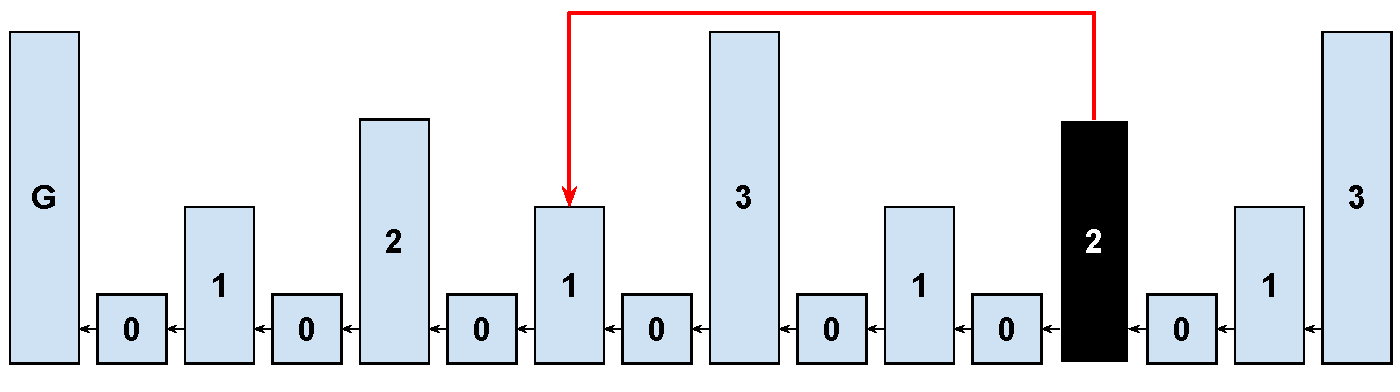
\includegraphics[width=0.9\columnwidth]{figures/simple_thorny.pdf}
	\end{center}
    \caption{A thorny pointer of an adversarial block, colored black, in an honest party's chain. The thorny block points to a $1$-superboock which is an ancestor
		$1$-superblock, but not \emph{the most recent ancestor} $1$-superblock.}
	\label{fig:skip_ancestor}
\end{figure}

As such, we conclude that the honest verifier comparing the honest superchain
against the adversarial superchain will reach the same conclusion in the velvet
case as he would have reached in the soft fork case: Because the honest
superchain in the velvet case contains the same amount of blocks as the honest
superchain in the soft fork case, but the adversarial superchain in the velvet
case contains fewer blocks than in the soft fork case, the comparison will
remain in favor of the honest party. As we will see in the next section, this
conclusion is far from straightforward.
